\section{Exemplos de Geodésicas}

Para ilustrar o conceito de geodésica, vamos exibi-las em algumas superfícies diferentes.

\subsection{Cilindro}

Para encontrar as geodésicas de um cilindro, utilizaremos a Proposição \ref{nao varia por isometria} e obte-las-emos por meio das geodésicas do plano.
Intuitivamente, está claro que as geodésicas em um plano são justamente os segmentos de reta nele contidos.
Para formalizar essa intuição, basta perceber que, dado um desses segmentos de retas, podemos facilmente parametrizá-lo localmente por uma curva de velocidade constante.
Com isso, sua aceleração é nula e, assim, perpendicular ao espaço tangente do plano em cada ponto.

Com esse conhecimento em mãos, pela Proposição \ref{nao varia por isometria} precisamos apenas de encontrar uma isometria entre o plano e o cilindro.
Felizmente, isso não é muito difícil, pois a parametrização usual do cilindro é uma isometria.

Denotando por \( C \defeq \mathbb{S}^{ 1 } \times \R = \left\{ ( x, y, z ) \in \R^{ 3 } : x^2 + y^2 = 1 \right\} \) o cilindro, por \( S \) o plano em \( \R^{ 3 } \) correspondente a \( z = 0 \) e por \( U \defeq \left\{ ( x, y, 0 ) \in S : - \pi < x < \pi \right\} \) o retângulo entre \( -\pi \) e \( \pi \), nossa isometria é \( f : U \subseteq S \to f ( U ) \subseteq C \) dada por
\begin{equation*}
    f ( x, y, z ) = ( \cos x, \sen x, y )
.\end{equation*}

Logo, as geodésicas no cilindro são as imagens de segmentos de reta por \( f \).
Ilustramos algumas delas na Figura \ref{geodesicas cilindro}.

\begin{figure}[htb]
    \begin{center}
        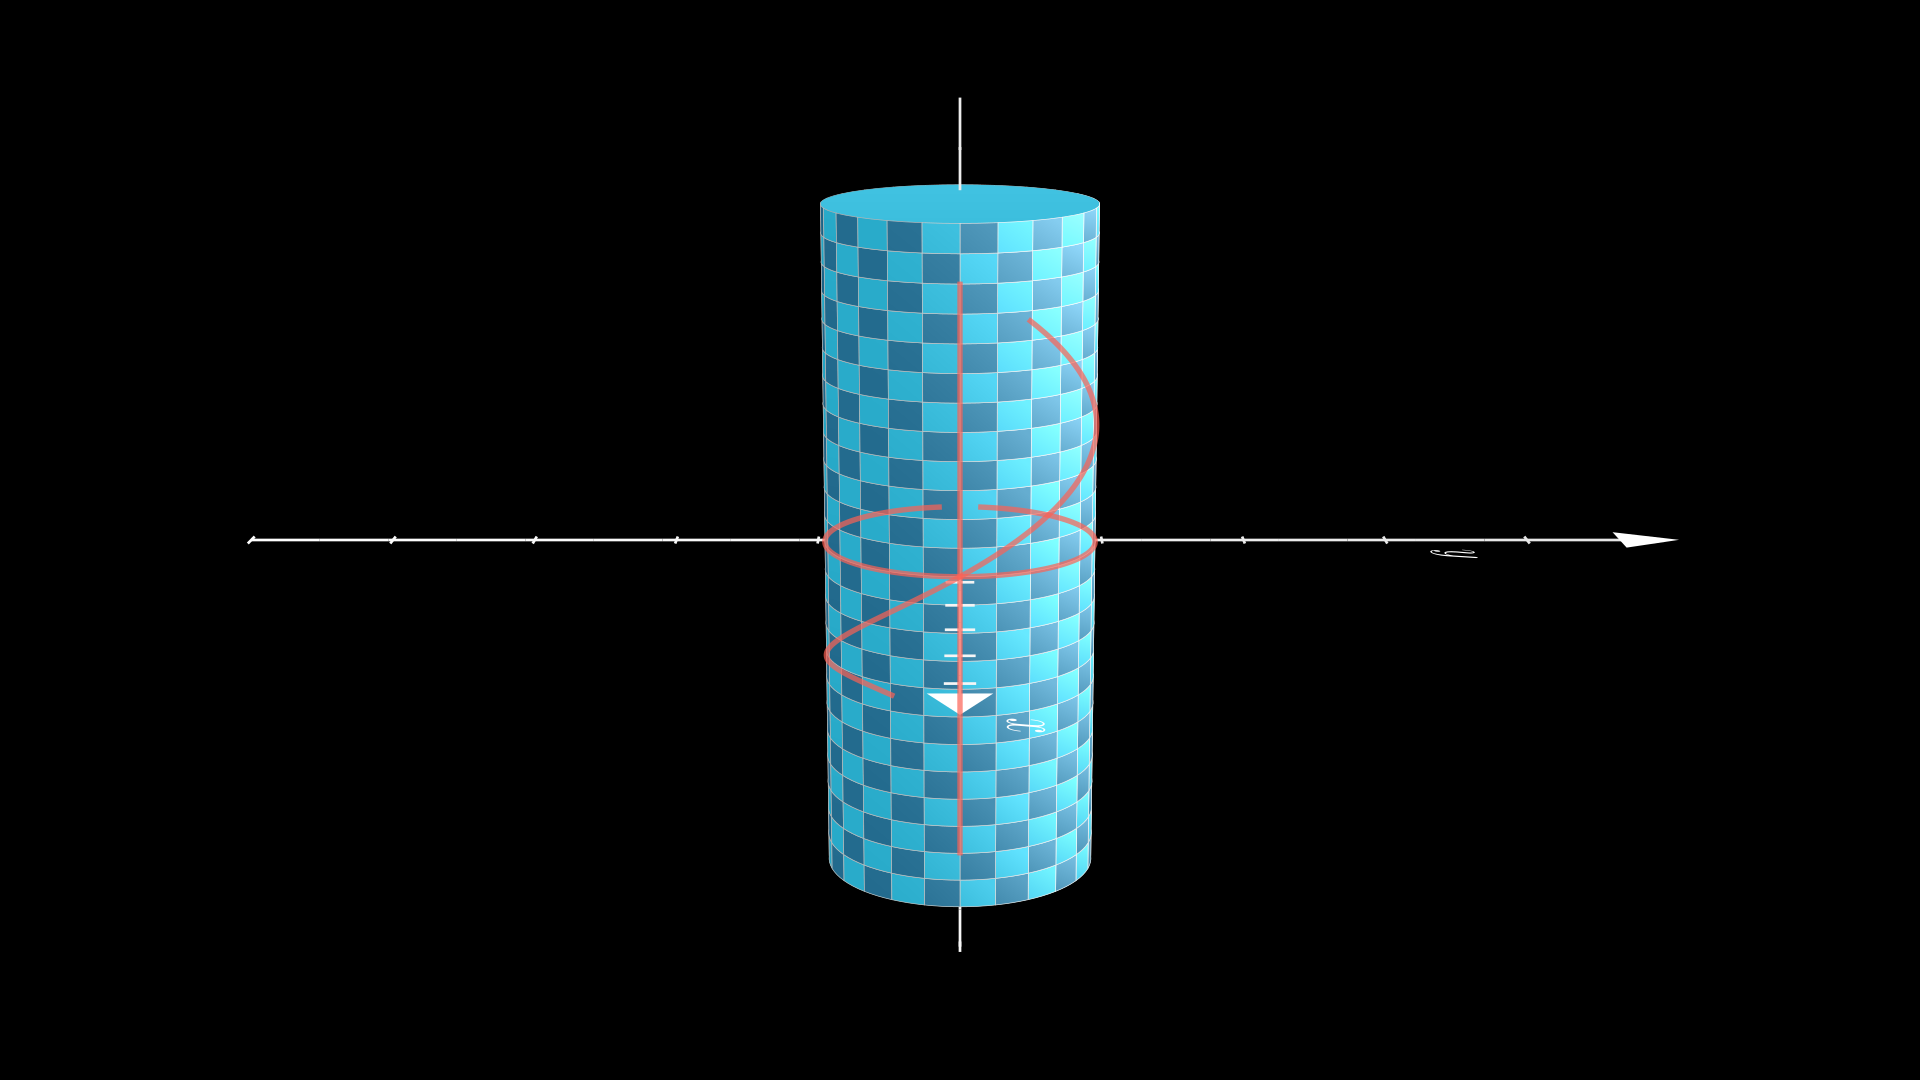
\includegraphics[width=.5\textwidth]{cilindro-1}
        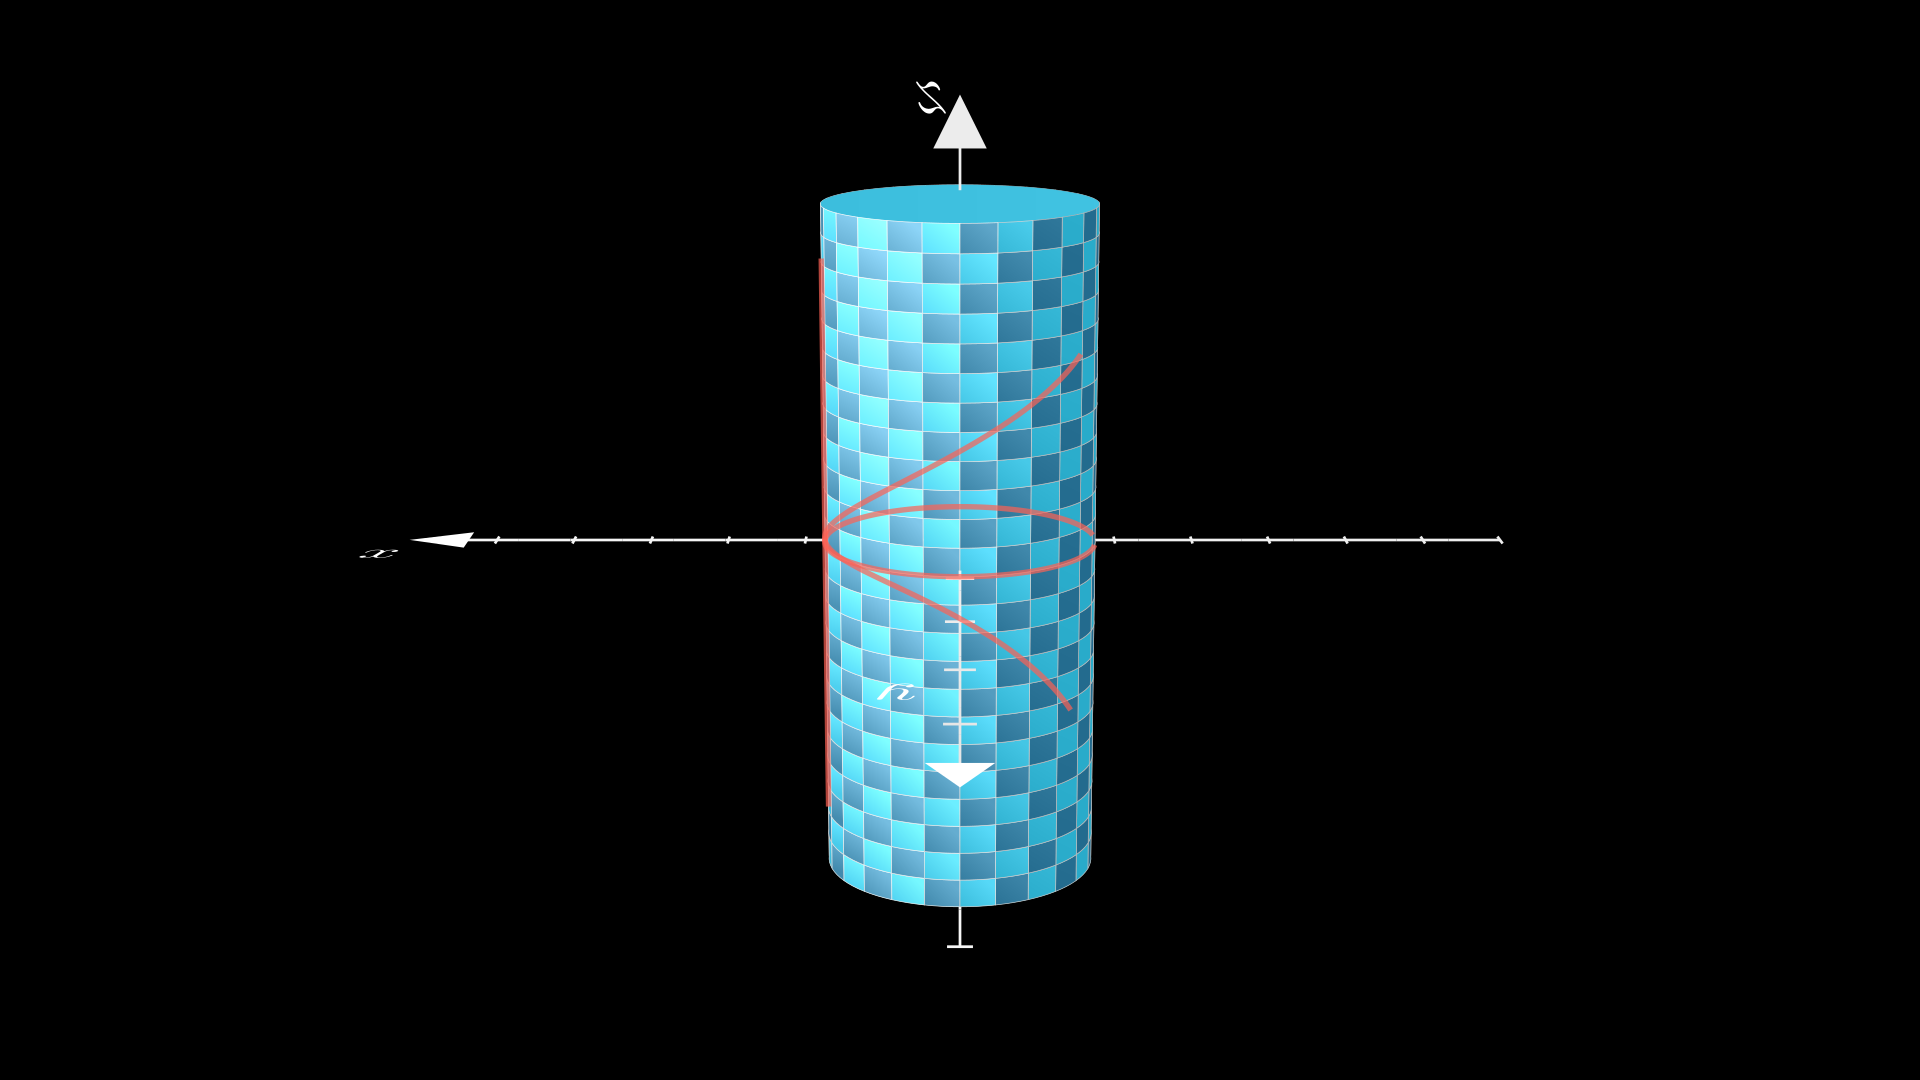
\includegraphics[width=.5\textwidth]{cilindro-2}
        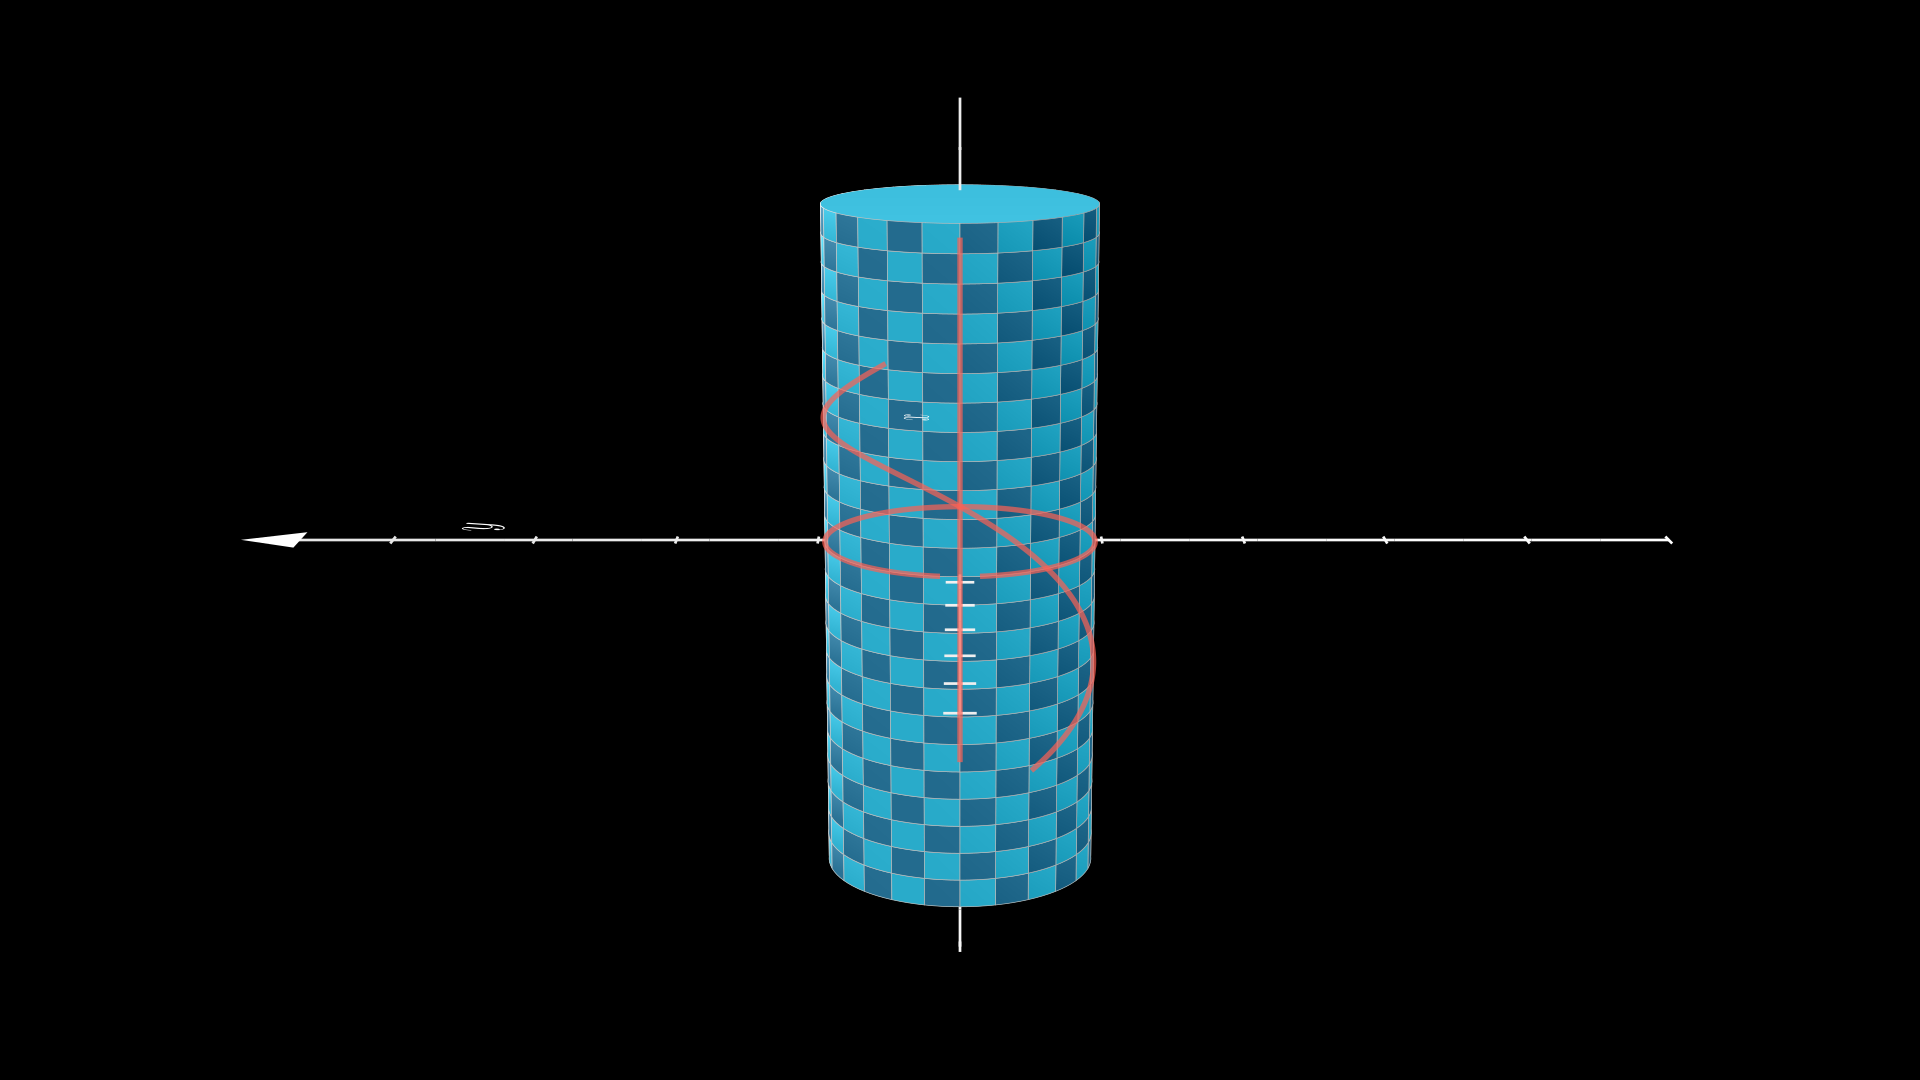
\includegraphics[width=.5\textwidth]{cilindro-3}
        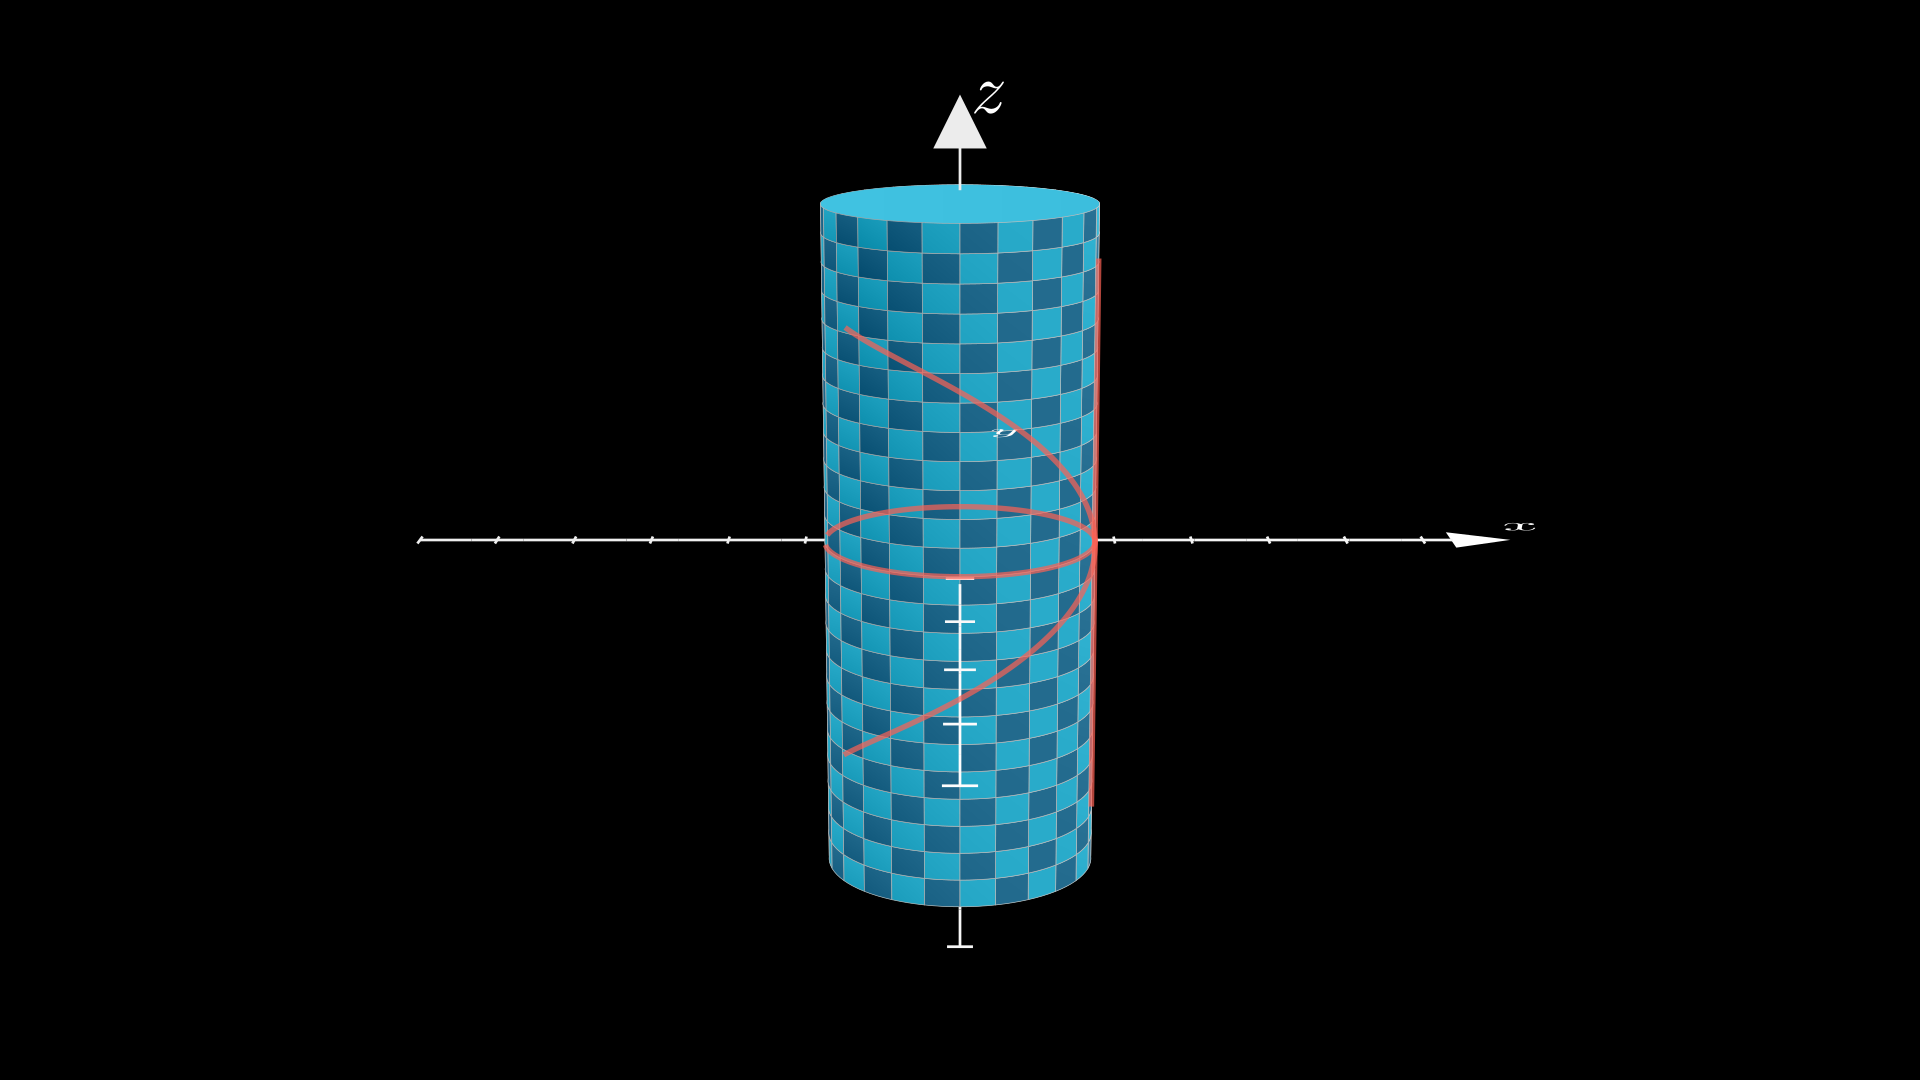
\includegraphics[width=.5\textwidth]{cilindro-4}
    \end{center}
    \caption{Três tipos de geodésicas no cilindro, sob diferentes pontos de vista.}
    \label{geodesicas cilindro}
\end{figure}

\subsection{Esfera}

Para encontrar as geodésicas da esfera, podemos resolver o sistema de equações diferenciais apresentado em (\ref{difeq}), ou podemos prosseguir por um argumento mais geométrico, como a seguir.
Primeiramente, perceba que o grande arco \( C \) de \( \mathbb{S}^{ 2 } \) parametrizado por \( \gamma ( \theta ) = ( \cos ( \theta ), \sen ( \theta ), 0 ) \) tem aceleração \( \gamma'' ( \theta ) = - ( \cos ( \theta ), \sen ( \theta ) ) = - \gamma ( \theta ) \).
Como \( T_{ \gamma ( t ) } \mathbb{S}^{ 2 } = \left\{ \gamma ( t ) \right\}^{ \perp } \), temos que \( \gamma'' ( t ) \) é perpendicular ao espaço tangente em \( \gamma ( t ) \) para todo \( t \).
Logo, \( \gamma ( t ) \) descreve uma geodésica na esfera.
Agora, como todo grande arco de \( \mathbb{S}^{ 2 } \) é a imagem de \( C \) por uma rotação (a qual, por ser uma transformação linear ortogonal, é isometria), concluímos da Proposição \ref{nao varia por isometria} concluímos que todo grande arco de \( \mathbb{S}^{ 2 } \) é uma geodésica.
Alguns deles estão representados na Figura \ref{geodesicas esfera}.

\begin{figure}[htb]
    \begin{center}
        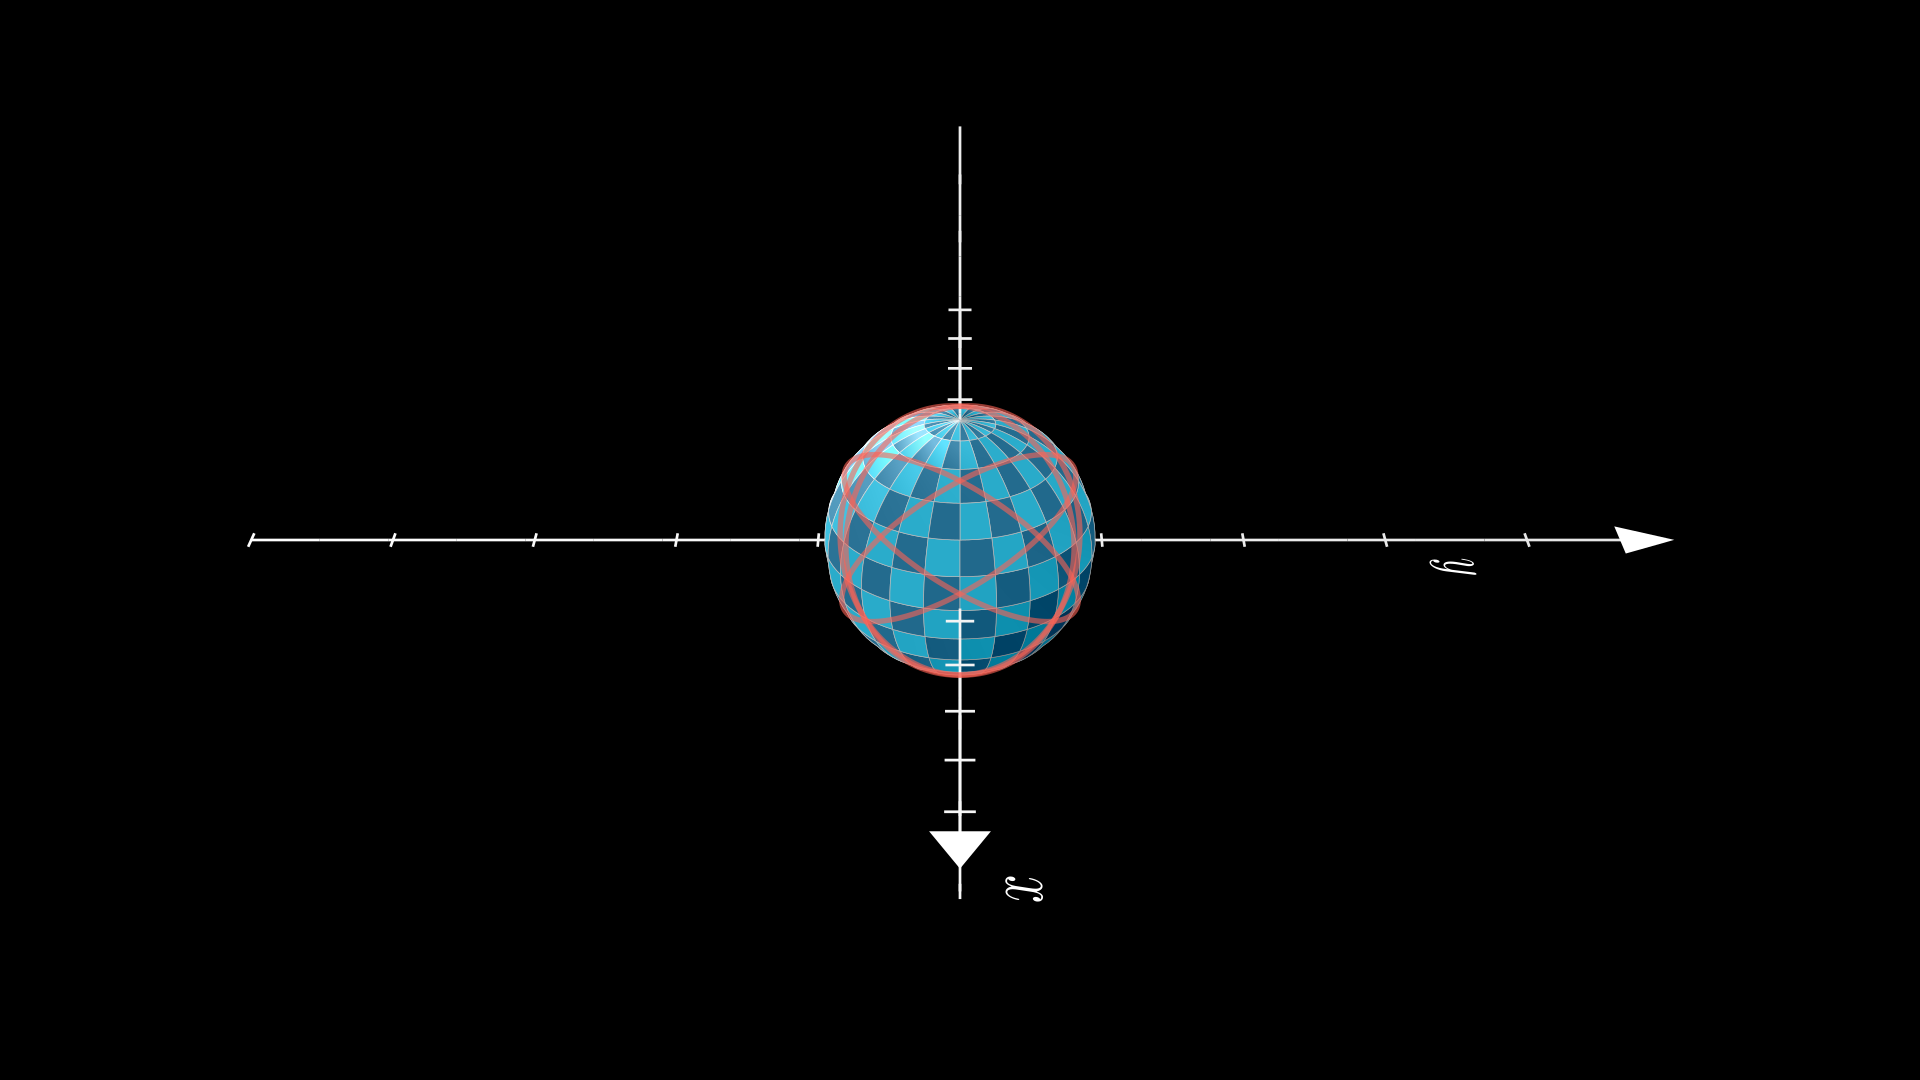
\includegraphics[width=.7\textwidth]{esfera-1}
        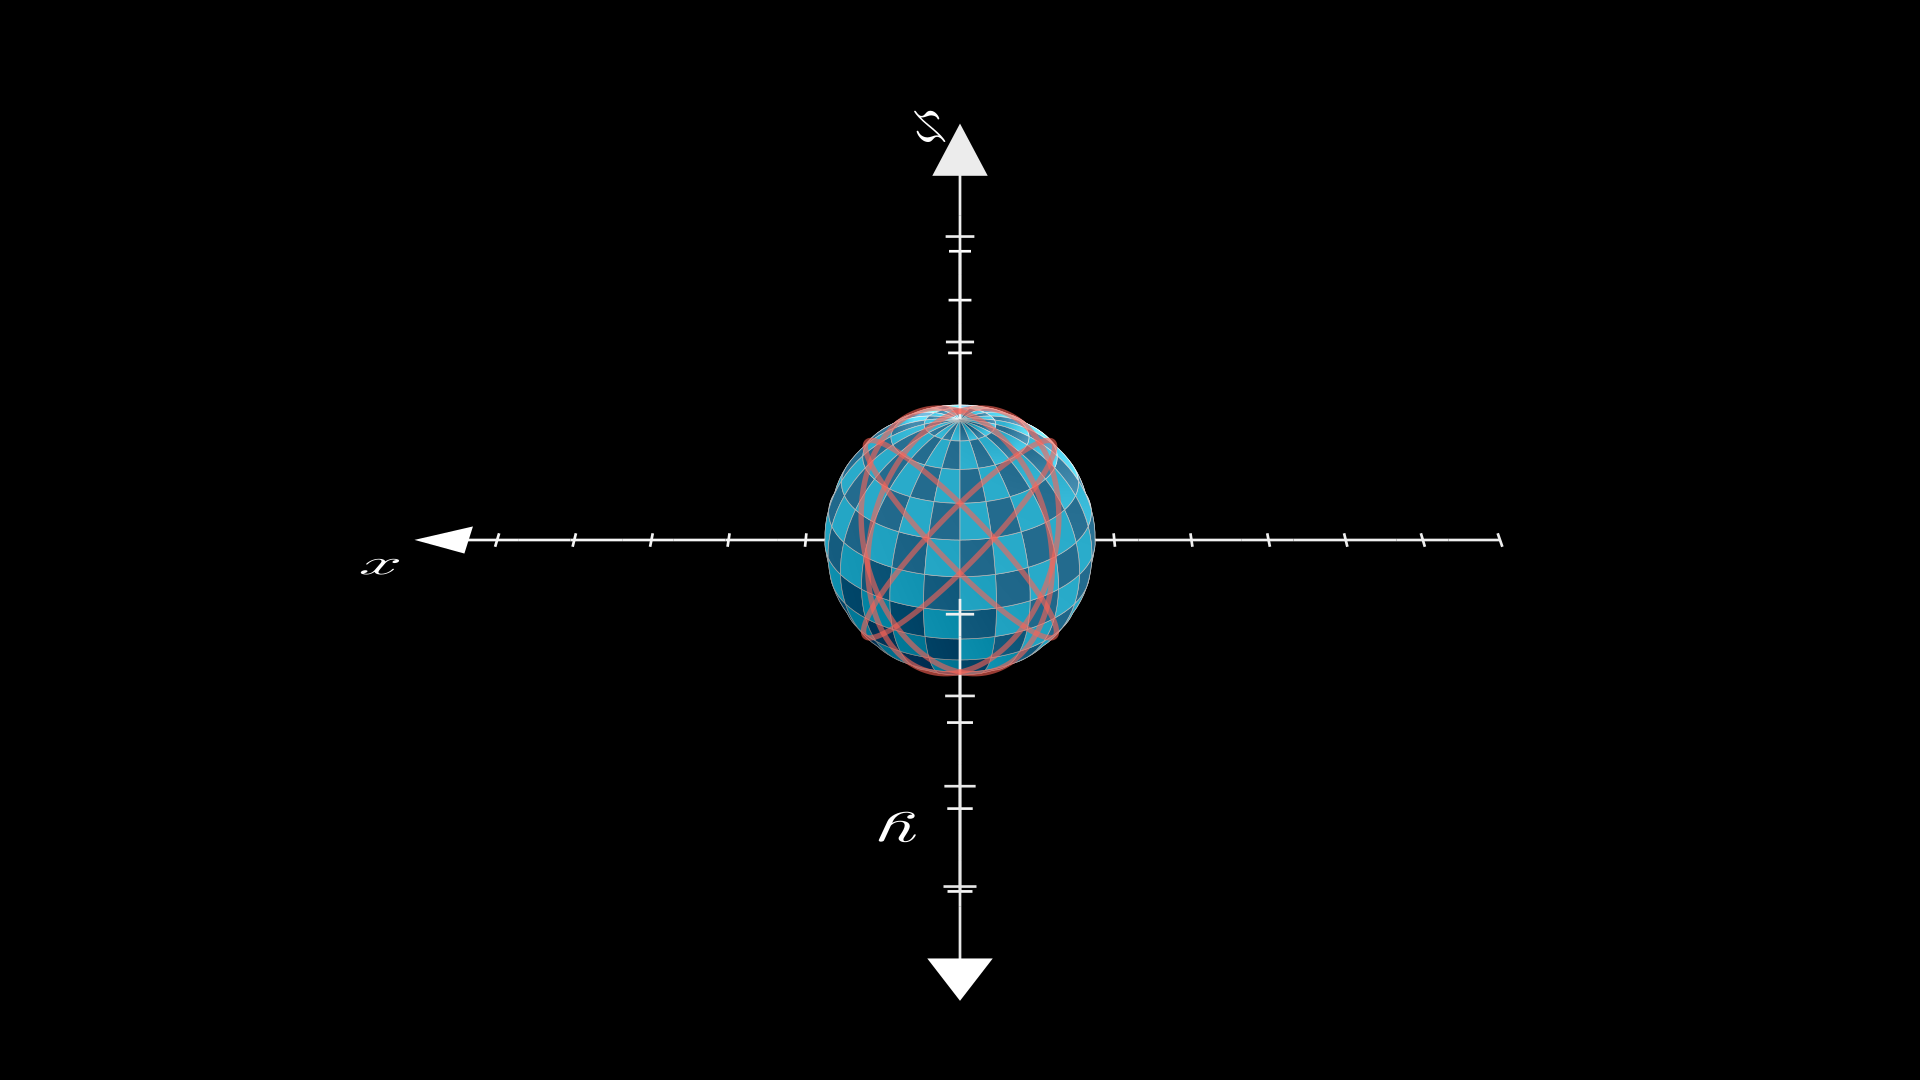
\includegraphics[width=.7\textwidth]{esfera-2}
    \end{center}
    \caption{Alguns grandes arcos em \( \mathbb{S}^{ 2 } \), sob dois pontos de vista.}
    \label{geodesicas esfera}
\end{figure}
